\documentclass[12pt,a4paper]{article}
\usepackage[utf8]{inputenc}
\usepackage{graphicx}
\usepackage{float}
\usepackage{subcaption}
\usepackage[margin=1in]{geometry}
\usepackage{hyperref}  
\hypersetup{
  pdfborder = {0 0 0}
}
\usepackage[
backend=biber,
style=alphabetic,
]{biblatex}

\addbibresource{radio.bib}

\graphicspath{{./Pictures/}}
\DeclareGraphicsExtensions{.pdf,.jpeg,.jpg,.png}

\usepackage{amsmath} % equations
\usepackage{fancyhdr} % nicer page header
\usepackage{listings} % For inclusion of code


\setlength{\parindent}{0pt} % no paragraph indents
\setlength{\parskip}{1em} % paragraphs separated by one line

\newcommand\experiment{Experiment Radio astronomy} %%%%% experiment name
\newcommand\groupno{Group 3+12}       %%%%% group number
\newcommand\names{Pratyush Singh,\\
                  Proshmit Dasputpa,\\
                  Dhruv Nahar}        %%%%% full names
\newcommand\expdate{25/03/2025}    %%%%% date of experiment day

\begin{document}
\begin{titlepage}
   \begin{center}
        \vspace*{3cm}
        \Huge{\experiment}
				
        \vspace{0.5cm}
        \LARGE{Lab course protocol}
				
        \vspace{3 cm}
        \Large{\groupno}
				
        \vspace{0.25cm}
        \large{\names}
				
        \vspace{2 cm}
        \Large{\expdate}
				
        \vspace{0.25 cm}
        \Large{Advanced lab course in astronomy\\
				Eberhard Karls Universit\"at T\"ubingen}
				
				\vspace{0.1 cm}
        \Large{WiSe 2024/25}
				
       \vfill
    \end{center}
\end{titlepage}

\pagestyle{fancy}
\fancyhf{}
\setlength{\headheight}{14.5pt}
\lhead{\groupno; \experiment}

% \section*{Abstract}
% This is optional, but never longer than half a page.

\tableofcontents
\newpage

\setcounter{page}{1}
\pagestyle{fancy}
\fancyhf{}
\rhead{\thepage}
\lhead{\groupno; \experiment}

\section{Introduction}\label{sec:intro} % labels allow references, particularly important for figures and tables


\section{Theory}
\label{sec:theory}
  \subsection{The Sun}
  \subsection{The Milky Way}
    \subsubsection{Doppler Effect}
    \subsubsection{Milkay Way Rotation}
    \subsubsection{Mass Estimate}
    % MORE IF NEEDED

\section{Experiment}
    \subsection{The Telescope}
        The radio telescope at Sand 1, Tübingen is a parabolic antenna with a diameter of 2.3 m. At the 21 cm Hydrogen line, it has a
        resolution of $5^\circ$. The telescope is controlled using the qradio software on a computer attached to it. \\
        The telescope can either be operated as a bolometer (measuring the total power of radio signal) or as a spectrometer. For the first case,
        the measured signal is compared to the calibration source (`noise diode') located in the middle of the dish. For spectrometry, the power is measured 
        together for the source and the background such that radio noise from human sources, sky emissions and the continuum emission of the source can be subtracted.

        \begin{figure}[H]
            \centering
            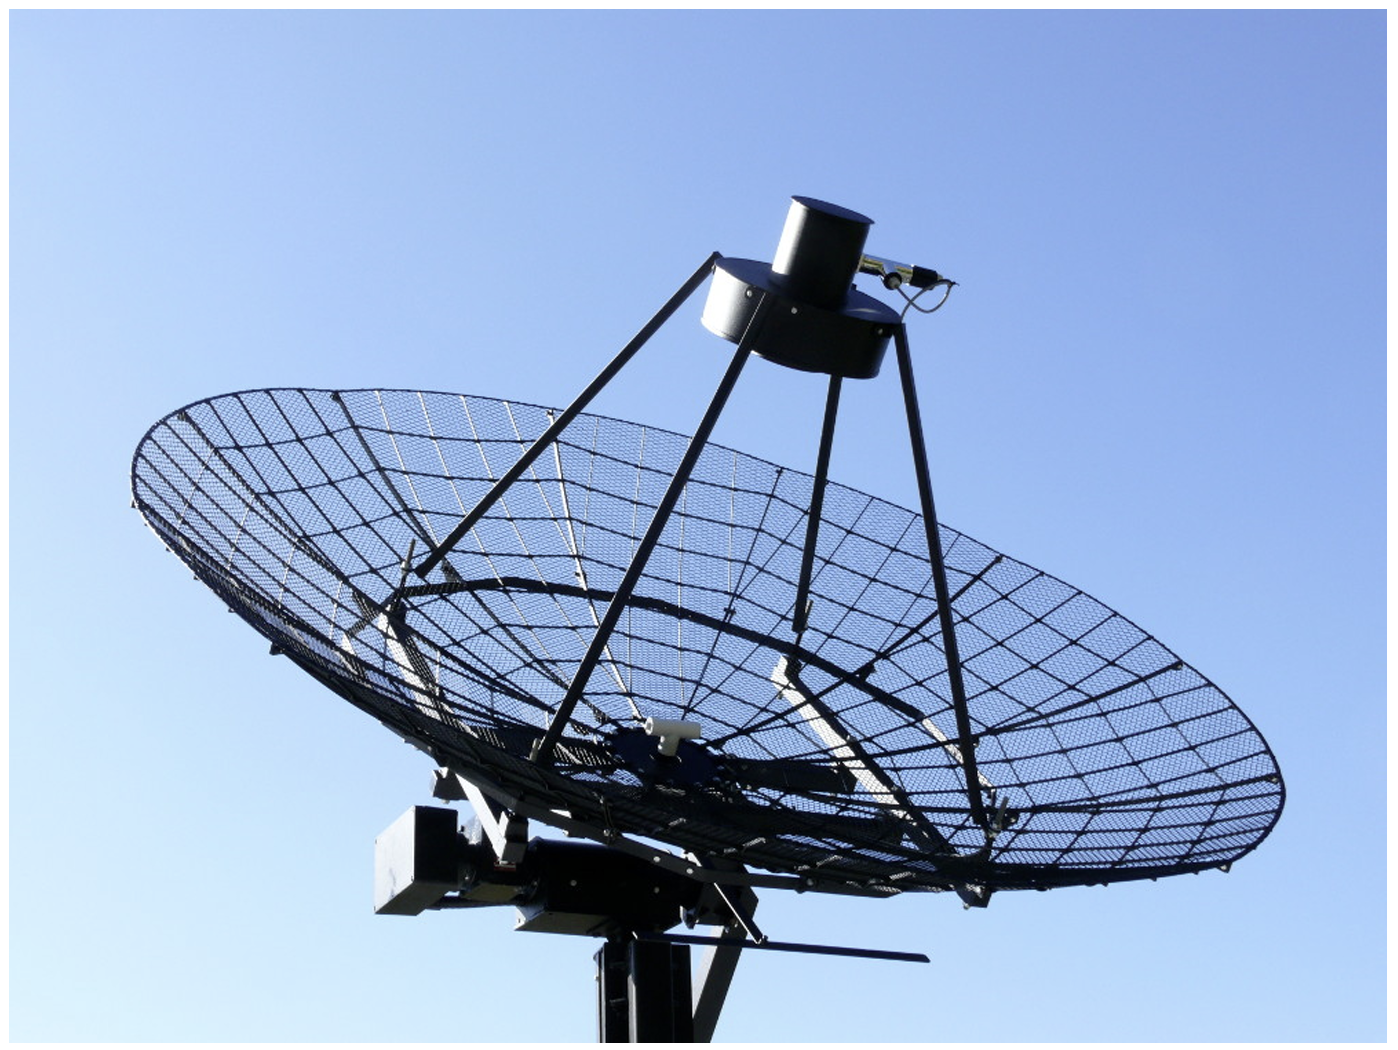
\includegraphics[width=0.5\textwidth]{telescope.png}
            \caption{Radio telescope at Sand 1, Tübingen}
            \label{fig:telescope}
        \end{figure}

        The telescope is on a Alt-Az mount. Using the computer, the telescope can be moved by specifying galactic, equatorial and other coordinate systems.
    \subsection{Observations}
            To start the observations, first a restart of the computer is required. The program qradio is started with the following configurations:\ref{fig:qradio_config}
            \begin{figure}[H]
                \centering
                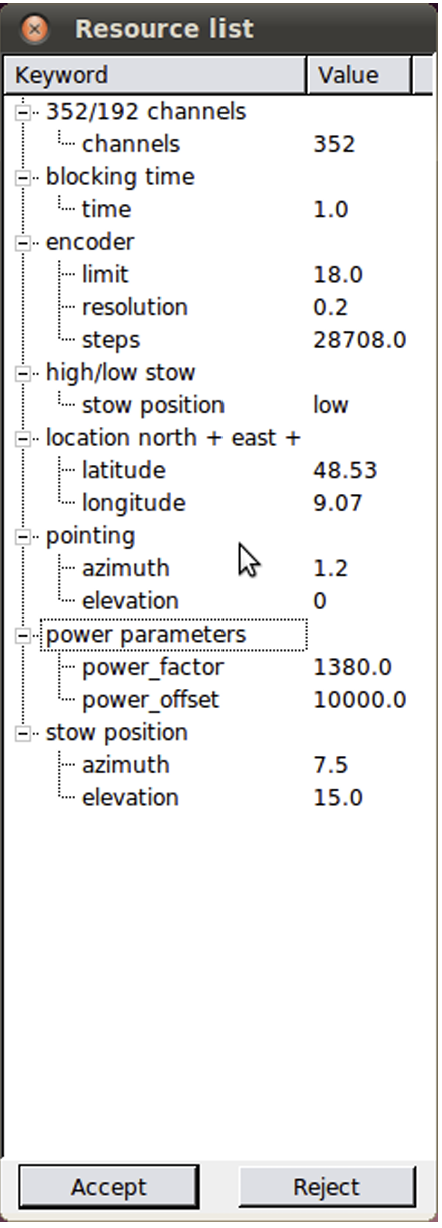
\includegraphics[width=0.15\textwidth]{qradio_config.png}
                \caption{qradio configuration. All the shown values much match}
                \label{fig:qradio_config}
            \end{figure} 

            Now using the GUI, different parameters are set for the observations of the sun and the Milky Way.

            \begin{figure}[H]
                \centering
                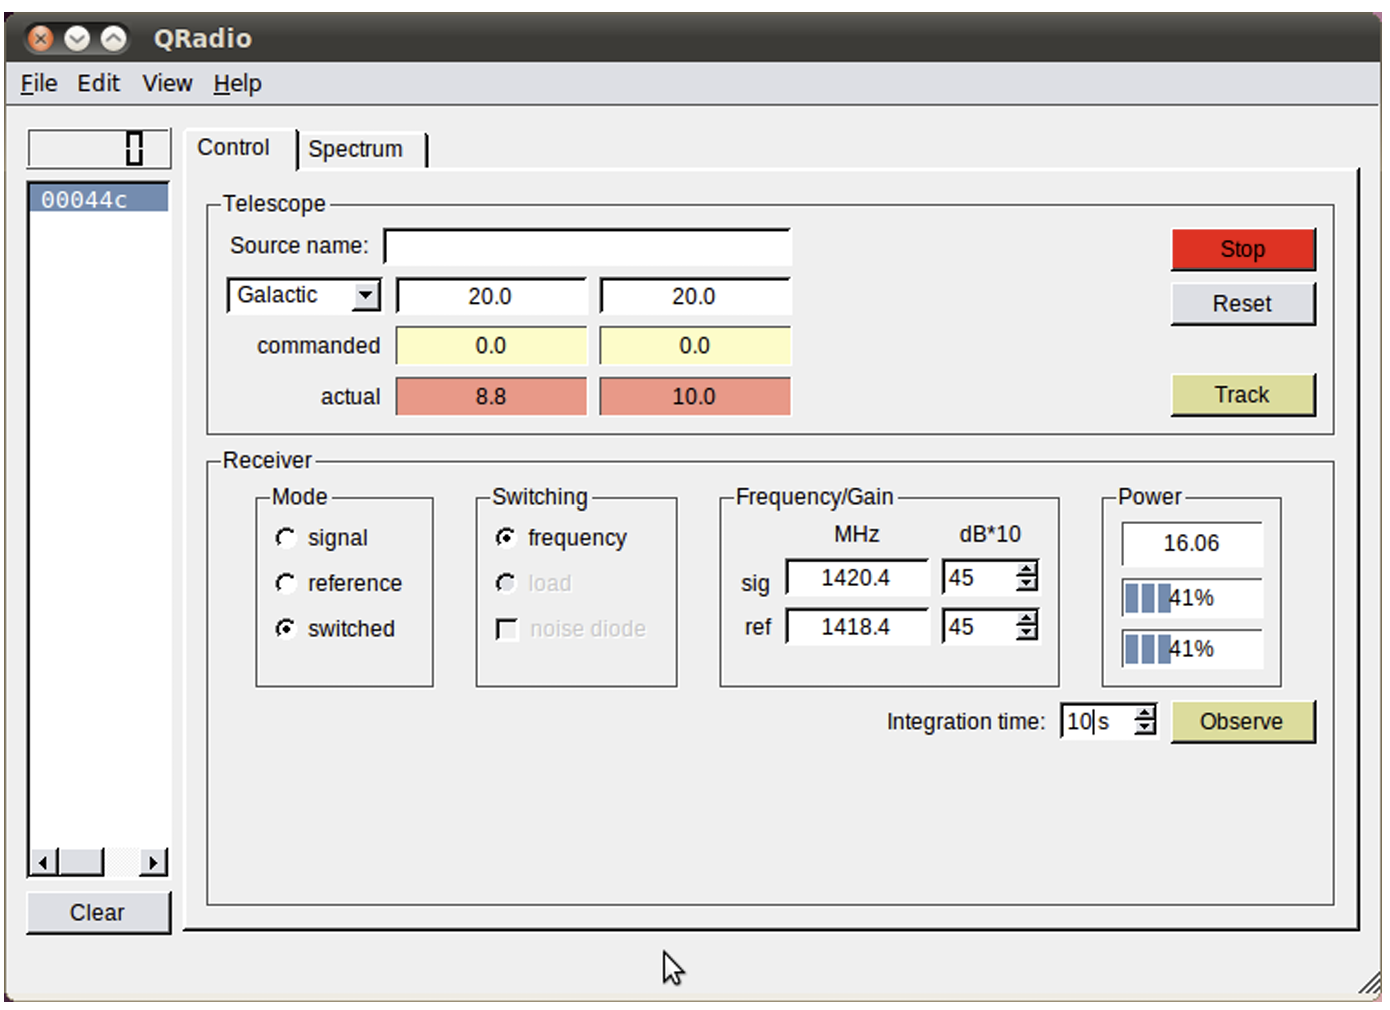
\includegraphics[width=0.5\textwidth]{qradio_gui.png}
                \caption{the qradio GUI}
                \label{fig:qradio_gui}
            \end{figure}
        \subsubsection{Observation of the Sun}
        \subsubsection{Observation of the Milky Way Disk}
            To observe the Milky Way, the following parameters were set:
            \begin{enumerate}
                \item In the \textit{receiver} box, \textit{Mode} is set as `switched' with \textit{Switching} set to `frequency'.
                \item In the \textit{Frequency/Gain} box, $dB*10$ is adjusted such that both signal and reference levels are about $30\%$. We set the it to 30.
                \item We set the coordinates in the \textit{Telescope} box by first setting the coordinate system as `Galactic'. The coordinates are then entered in degrees.
                \item By clicking on \textit{Track} the telescope will move to the required position and will track that coordinate over time.
                \item The spectrum is observed by setting an \textit{integration time} of 10 seconds and by clicking \textit{observe}. The spectrum can then be inspected in the \textit{Control} tab and can be saved.
                \item Next we track and get the spectrum for several sets of coordinates. 
            \end{enumerate}
            
            To choose the coordinates to observe, we first start with part of the disk that is closest to setting in the west anc continue eastward. Spectrums are obtained for $l=25^\circ,30^\circ,40^\circ \dots 80^\circ, 89^\circ$ as b is kept constant at $b=0^\circ$ since we are observing the centre of the disk. \\

            Background measurements are taken at $l=30^\circ,50^\circ,80^\circ$ and $b=30^\circ$ to be subtracted from the previous set of observations.

    \subsection{Data Analysis}

\section{Conclusions}

\printbibliography     
\appendix
\section{Appendix}

\end{document}

